\documentclass[journal,twoside,web]{ieeecolor}
\usepackage{generic}
\usepackage{cite}
\usepackage{amsmath,amssymb,amsfonts}
\usepackage{algorithmic}
\usepackage{graphicx}
\usepackage{algorithm,algorithmic}
\usepackage{hyperref}
\hypersetup{hidelinks=true}
\usepackage{textcomp}
\usepackage{array}


\newcolumntype{L}[1]{>{\raggedright\arraybackslash}m{#1}} % 左对齐 + 垂直居中 + 固定宽
\newcolumntype{Y}{>{\raggedright\arraybackslash}X}       % 左对齐 + 自动伸缩
  % 左对齐+自动伸缩

\usepackage{tabularx} 
\usepackage{multirow}
\usepackage{booktabs}
\def\BibTeX{{\rm B\kern-.05em{\sc i\kern-.025em b}\kern-.08em
    T\kern-.1667em\lower.7ex\hbox{E}\kern-.125emX}}
\markboth{\hskip25pc IEEE TRANSACTIONS AND JOURNALS TEMPLATE}
{Author \MakeLowercase{\textit{et al.}}: Title}
\begin{document}
\title{Reflex-Informed Deep Reinforcement Learning for Musculoskeletal Gait Generation}
\author{First A. Author, \IEEEmembership{Fellow, IEEE}, Second B. Author, and Third C. Author Jr., \IEEEmembership{Member, IEEE}
\thanks{This paragraph of the first footnote will contain the date on 
which you submitted your paper for review. It will also contain support 
information, including sponsor and financial support acknowledgment. For 
example, ``This work was supported in part by the U.S. Department of 
Commerce under Grant 123456.'' }
\thanks{The next few paragraphs should contain 
the authors' current affiliations, including current address and e-mail. For 
example, First A. Author is with the National Institute of Standards and 
Technology, Boulder, CO 80305 USA (e-mail: author@boulder.nist.gov). }
\thanks{Second B. Author Jr. was with Rice University, Houston, TX 77005 USA. He is 
now with the Department of Physics, Colorado State University, Fort Collins, 
CO 80523 USA (e-mail: author@lamar.colostate.edu).}
\thanks{Third C. Author is with 
the Electrical Engineering Department, University of Colorado, Boulder, CO 
80309 USA, on leave from the National Research Institute for Metals, 
Tsukuba, Japan (e-mail: author@nrim.go.jp).}}

\maketitle

\begin{abstract}
These instructions give you guidelines for preparing papers for 
IEEE Transactions and Journals. Use this document as a template if you are 
using \LaTeX. Otherwise, use this document as an 
instruction set. The electronic file of your paper will be formatted further 
at IEEE. Paper titles should be written in uppercase and lowercase letters, 
not all uppercase. Avoid writing long formulas with subscripts in the title; 
short formulas that identify the elements are fine (e.g., "Nd--Fe--B"). Do 
not write ``(Invited)'' in the title. Full names of authors are preferred in 
the author field, but are not required. Put a space between authors' 
initials. The abstract must be a concise yet comprehensive reflection of 
what is in your article. In particular, the abstract must be self-contained, 
without abbreviations, footnotes, or references. It should be a microcosm of 
the full article. The abstract must be between 150--250 words. Be sure that 
you adhere to these limits; otherwise, you will need to edit your abstract 
accordingly. The abstract must be written as one paragraph, and should not 
contain displayed mathematical equations or tabular material. The abstract 
should include three or four different keywords or phrases, as this will 
help readers to find it. It is important to avoid over-repetition of such 
phrases as this can result in a page being rejected by search engines. 
Ensure that your abstract reads well and is grammatically correct.
\end{abstract}

\begin{IEEEkeywords}
Enter key words or phrases in alphabetical order, separated by commas. Using the IEEE Thesaurus can help you find the best standardized keywords to fit your article. Use the thesaurus access request form for free access to the IEEE Thesaurus: \underline{https://www.ieee.org/publications/services/thesaurus-}\discretionary{}{}{}\underline{access-page.com.}
\end{IEEEkeywords}

\section{Introduction}
\label{sec:introduction}

% 人类下肢运动是一种高度复杂且高鲁棒性的运动形式，其神经控制系统具有明显的层级特征：脊髓反射通路负责快速反馈，而上位中枢调控节律与目标。近年来，肌骨（MSK）模型被广泛用于人类运动仿真。该类模型在生理层面耦合了骨骼动力学与肌肉生物力学，可由肌肉激活预测关节力矩与运动轨迹，为理解神经控制机制提供了可解释的建模平台。基于此模型研究运动的稳定性与生理合理性，对于康复工程、仿生机器人与虚拟人运动生成均具有重要意义。然而，如何在保证生理合理性的前提下生成稳定且能量高效的运动，仍是当前研究的关键挑战。

% 为实现具有生理合理性的稳定步态生成，研究者提出了多种控制策略。现有控制策略主要包括反射控制、中央模式发生器（CPG）以及肌肉协同（muscle synergy）方法。反射控制以生物反射机制为基础，通过模拟肌梭、腱器官及足底触觉等反馈通路，构建局部感知–反应式控制律（如 Geyer 与 Herr 提出的脊髓反射模型），能够在特定条件下生成稳定的行走模式，并较好地解释人类步态的神经调控机制。然而，这类模型通常依赖经验参数或离线优化，对任务或环境变化的响应能力有限。CPG利用神经振荡网络产生节律性输出，并在外部反馈的调节下驱动周期运动。该模型能够有效生成连续的步态节律，但在应对扰动和地形变化时，往往缺乏快速的适应与稳定恢复能力。此外，部分研究基于**肌肉协同（muscle synergy）**理论，通过降低肌肉激活空间的维度，将复杂的肌群控制简化为若干协同模式的线性组合。这类方法在一定程度上提高了计算效率，并揭示了肌肉协调的内在结构，但其协同模式多来源于数据驱动分解或经验假设，缺乏在线调节与生理反馈机制的支持。

% 随着深度强化学习（Deep Reinforcement Learning, DRL）的发展，出现了大量基于策略学习的运动生成研究。此类方法通过与仿真环境的交互学习控制策略，能够在端到端框架下实现行走、跑步等多种运动形式。尽管强化学习在运动控制任务中展现出强大的策略优化能力，但其在神经肌骨系统中的应用仍面临显著挑战：高维控制变量、强耦合的肌肉动力学以及缺乏生理约束，使得策略学习过程容易陷入非生理、低效率的探索。与此形成对比，生理启发的反射机制为运动控制提供了丰富的结构先验，能够在局部反馈层面保证稳定与可解释性。因此，本文提出了一种Reflex-Informed Deep Reinforcement Learning 框架,在 off-policy 的 Actor–Critic 学习结构下引入生理反射的神经控制规律。该框架以反射模型作为低层控制结构，Actor 网络生成反射参数候选，Critic 网络根据运动性能评估策略价值，并通过基于概率推断的策略优化算法（Maximum a Posteriori Policy Optimization, MPO）实现稳定的策略更新,使策略学习过程在生理合理的空间中进行约束与优化。该方法在保证反射控制稳定性的同时，提升了参数调整的效率与全局性能，从而在仿真步态生成中展现出更稳定且能量合理的运动特征。


% 本文的主要贡献如下：
% （1）从神经启发视角出发，提出 Reflex-Informed DRL 框架，在 MSK 模型上实现结构化神经反馈控制，实现稳定、可解释的学习；
% （2）采用并论证 Maximum a Posteriori Policy Optimization (MPO) 在高维肌骨系统中的适用性，实现反射参数的高效更新与稳定策略学习；
% （3）基于公开步态数据验证框架的生理一致性，模型生成的关节角度在不同速度下与健康受试者步态趋势一致，证明了该方法在生理合理性与学习效率上的优势。
% 本文余下部分结构如下：第二节介绍方法原理及模型设计；第三节描述实验设置与评估指标；第四节展示结果并进行分析；第五节总结全文与展望。


\IEEEPARstart{H}{uman} gait is a highly complex yet robust form of motion, characterized by a hierarchical control architecture in which fast spinal reflex pathways regulate local feedback responses, while higher-level neural structures modulate movement rhythms and task goals over longer temporal scales. Neuromusculoskeletal (NMSK) models, together with their simplified musculoskeletal variants, have therefore been widely adopted for the dynamic simulation of human locomotion, as they explicitly couple skeletal dynamics with muscle biomechanics and physiological control mechanisms. Such models provide an interpretable framework for investigating the neural regulation of human movement and are particularly valuable in applications where physiological plausibility and closed-loop stability are essential, such as rehabilitation engineering, bionic robotics, and computer animation. Despite these advantages, achieving stable and energy-efficient gait in NMSK systems remains challenging in practice. In many existing models, locomotion performance critically depends on carefully tuned control parameters, whose effects are highly sensitive to the complex interactions between sensory feedback, musculoskeletal dynamics, and environmental conditions. As a result, current approaches often rely on manual tuning or offline search, making it difficult to develop control strategies that are systematic, reproducible, and scalable in closed-loop locomotion control.

To address the difficulty of tuning control parameters in neuromusculoskeletal locomotion, a variety of biologically inspired control strategies have been proposed, including reflex-based control, central pattern generators (CPG), and muscle synergy-based approaches. Reflex-based control models encode local sensory–motor feedback loops inspired by spinal reflex mechanisms, enabling stable and physiologically interpretable gait generation. However, their performance typically depends on a large number of control parameters that are strongly coupled with musculoskeletal dynamics, and are often determined through manual tuning or offline optimization, which limits reproducibility and makes systematic scaling to different model configurations or conditions challenging.

CPG-based approaches employ coupled neural oscillators to generate rhythmic locomotion patterns with compact structure. While effective for rhythm generation, their parameters are primarily designed to ensure oscillatory stability and often require careful manual design and tuning, making systematic adjustment in closed-loop NMSK systems non-trivial.

Muscle synergy-based methods reduce the dimensionality of muscle coordination by representing activations as combinations of a limited number of synergies. Although this simplification alleviates some tuning complexity, synergy structures are  mainly derived from data-driven decompositions or empirical assumptions, and systematic adaptation in closed-loop control remains challenging.

%Reflex control is based on biological reflex mechanisms, simulating feedback pathways such as muscle spindles, Golgi tendon organs, and plantar tactile sensors to construct local perception–reaction control laws. Such models can generate stable walking patterns under specific conditions and effectively explain the neural regulation of human gait. However, these models typically rely on empirical parameters or offline optimization, which limits their scalability and makes systematic parameter adaptation within learning frameworks challenging. The CPG approach employs neural oscillatory networks to generate rhythmic outputs, driving periodic movements under the modulation of external feedback. This model can effectively produce continuous gait rhythms but often lacks rapid adaptability and stable recovery when facing perturbations or terrain variations. In addition, some studies have been inspired by the muscle synergy theory, which reduces the dimensionality of the muscle activation space by simplifying complex muscle group control into a linear combination of several coordinated patterns. Such methods improve computational efficiency to some extent and reveal the intrinsic structure of muscle coordination; however, their synergy patterns are mainly derived from data-driven decompositions or empirical assumptions, lacking online adaptability and the support of physiological feedback mechanisms.


Recently, with the rapid development of Deep Reinforcement Learning (DRL), a growing number of studies have explored DRL on motion generation based. These methods learn control policies through interactions with simulated environments, enabling the realization of various motion forms such as walking and running within an end-to-end framework. Although reinforcement learning demonstrates strong policy optimization capabilities in motor control tasks, end-to-end learning of actuator-level control commands in closed-loop NMSK locomotion remains difficult to stabilize and scale.Its application within NMSK systems still faces substantial challenges. The high-dimensional control variables, strongly coupled muscle dynamics, and the lack of physiological constraints often lead to the learning process to drift into non-physiological and inefficient exploration. 

Existing studies tend to emphasize either physiologically grounded control structure or learning-based optimization, but rarely consider both aspects simultaneously within a single neuromusculoskeletal locomotion framework. As a result, current approaches often involve trade-offs among physiological interpretability, closed-loop stability, and the ability to perform systematic parameter optimization.

Inspired by biological reflex mechanisms, this work propose a Reflex-informed Deep Reinforcement Learning framework that seeks to mitigate this trade-off. Rather than replacing physiologically based reflex control, the proposed approach treats reinforcement learning as a parameter inference mechanism for reflex modulation. This formulation enables systematic and data-driven adjustment of reflex parameters, addressing the limitations of manual tuning and end-to-end policy learning while preserving the stability and interpretability of reflex-based control.

Unlike existing approaches that either rely on hand-tuned reflex gains or employ end-to-end policy learning, the proposed method reformulates locomotion control as structured reflex modulation within a neuro-inspired hierarchical control framework, bridging biological motor control principles and data-driven policy optimization.The main contributions of this paper are as follows:

(1) A neuro-inspired hierarchical control framework for musculoskeletal gait generation is proposed. The method embeds physiologically grounded reflex mechanisms into a structured control architecture, where reinforcement learning operates as a high-level modulation mechanism over low-level feedback pathways, enabling stable and interpretable locomotion control.

(2) A low-dimensional and structured policy formulation for stable learning is introduced. By constraining policy optimization to a small set of reflex modulation parameters, the proposed approach reduces the effective control dimensionality and improves training stability compared with less structured control strategies.

(3) The proposed framework is validated in a musculoskeletal simulation environment, demonstrating stable and physiologically plausible gait generation with improved learning efficiency.

To the best of our knowledge, this is the first work that integrates a physiologically based reflex controller with an off-policy reinforcement learning algorithm within a musculoskeletal simulation framework. Unlike existing studies that either hand-tune reflex gains or employ end-to-end policy learning, our method optimizes reflex parameters through probabilistic policy inference, bridging the gap between biological motor control and deep reinforcement learning. The main contributions of this paper are as follows:

(1) A Reflex-Informed DRL framework is proposed from a neuro-inspired perspective, achieving structured neural feedback control on the MSK model for stable and interpretable learning.

(2) The MPO algorithm implemented within an off-policy Actor–Critic framework is adopted and validated for high-dimensional MSK control, demonstrating efficient reflex-parameter updates and stable policy learning.

(3) The proposed framework is validated using public gait data, where the generated joint trajectories across different speeds align with healthy gait trends, demonstrating advantages in both physiological plausibility and learning efficiency.

The remainder of this paper is organized as follows: Section II presents the methodology and model design; Section III describes the experimental setup and evaluation metrics; Section IV reports and analyzes the results; and Section V concludes the paper and outlines future work.



\section{Methodology}
\subsection{Overview of the Reflex-Informed DRL Framework}\label{formats}
Inspired by the hierarchical neurophysiological mechanisms of human locomotion, the proposed framework integrates a biologically grounded reflex controller with a DRL agent to achieve stable and physiologically plausible gait generation within a musculoskeletal simulation environment. As in Fig.~\ref{framwork}, the overall framework consists of three modules.
\textbf{(a)} The \textit{Actor--Critic Learning Module} optimizes the target policy via the MPO algorithm, where the critic network estimates the action-value function $Q(s,a)$, which is approximated by the neural network $q(s,a;\boldsymbol{\omega})$, and the actor network updates its policy parameters $\boldsymbol{\theta}_{\text{new}}$ to maximize the expected return. 
\textbf{(b)} The \textit{Agent--Environment Rollout Module} enables the behavior policy to interact with the environment, collecting experience tuples $(s_t, a_t, r_t, s_{t+1})$ that are stored in a replay buffer for off-policy sampling. 
\textbf{(c)} The \textit{Physiological Environment Module} integrates the RIC and the MSK model. 
The controller transforms the high-level policy outputs into physiologically meaningful muscle activations, while the MSK model simulates the resulting neuromuscular and skeletal dynamics.

This hierarchical integration bridges reflex-based control and DRL, combining the fast feedback regulation of biological reflexes with the high-level adaptability of policy learning, thereby enabling robust and physiologically grounded motion generation across different gait conditions. In the following sections, the proposed framework is detailed layer by layer,
including the physiological reflex–musculoskeletal model, the learning-based modulation mechanism,
and the policy optimization strategy.
\begin{figure}[!t]
\centerline{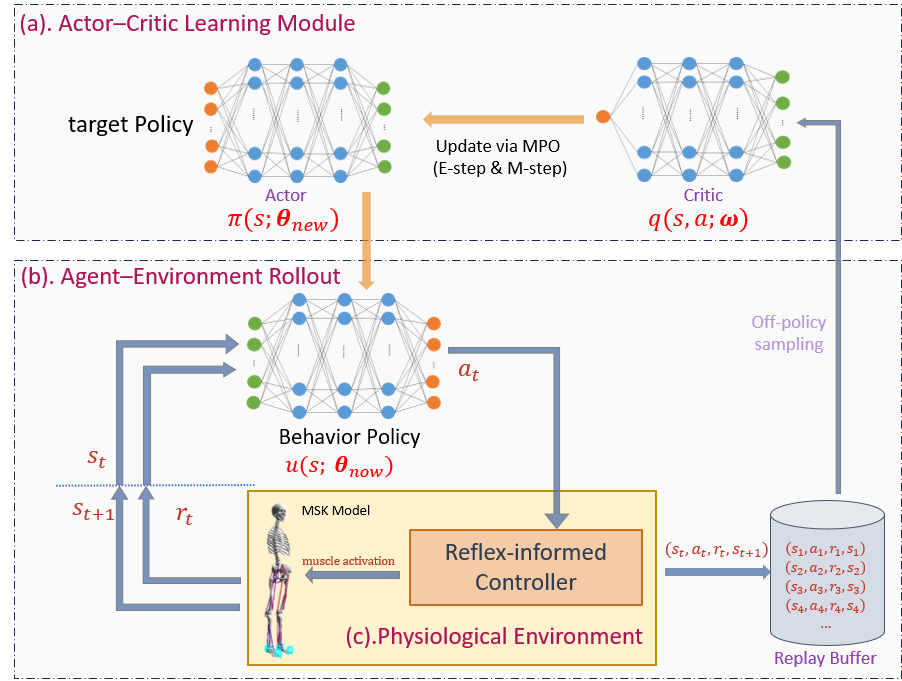
\includegraphics[width=\columnwidth]{framwork.png}}
\caption{Overview of the Reflex-Informed DRL Framework.}
\label{framwork}
\end{figure}


\subsection{Reflex-Informed Physiological Environment}\label{formats}
A physiologically consistent environment is essential for enabling the learning agent to acquire motor behaviors that align with human biomechanics. Therefore, the proposed framework introduces a reflex-informed physiological environment that bridges neural feedback regulation and musculoskeletal dynamics. This design provides a neurophysiologically grounded foundation for deep reinforcement learning, allowing policy optimization to proceed in a biologically interpretable and physiologically plausible manner.

\subsubsection{Neurophysiological Basis of Reflex Mechanisms}\label{formats}
In human locomotion, sensory feedback plays a crucial role in regulating muscle activation and joint stability.
The proprioceptive system relies primarily on two sensors: the muscle spindle, which detects changes in muscle length and velocity, and the Golgi tendon organ, which monitors muscle tension (Fig. 2).
These feedback signals are transmitted through spinal pathways to modulate motor neuron excitability, forming the physiological basis of reflex control that maintains balance and smooth gait transitions.

\begin{figure}[!t]
\centerline{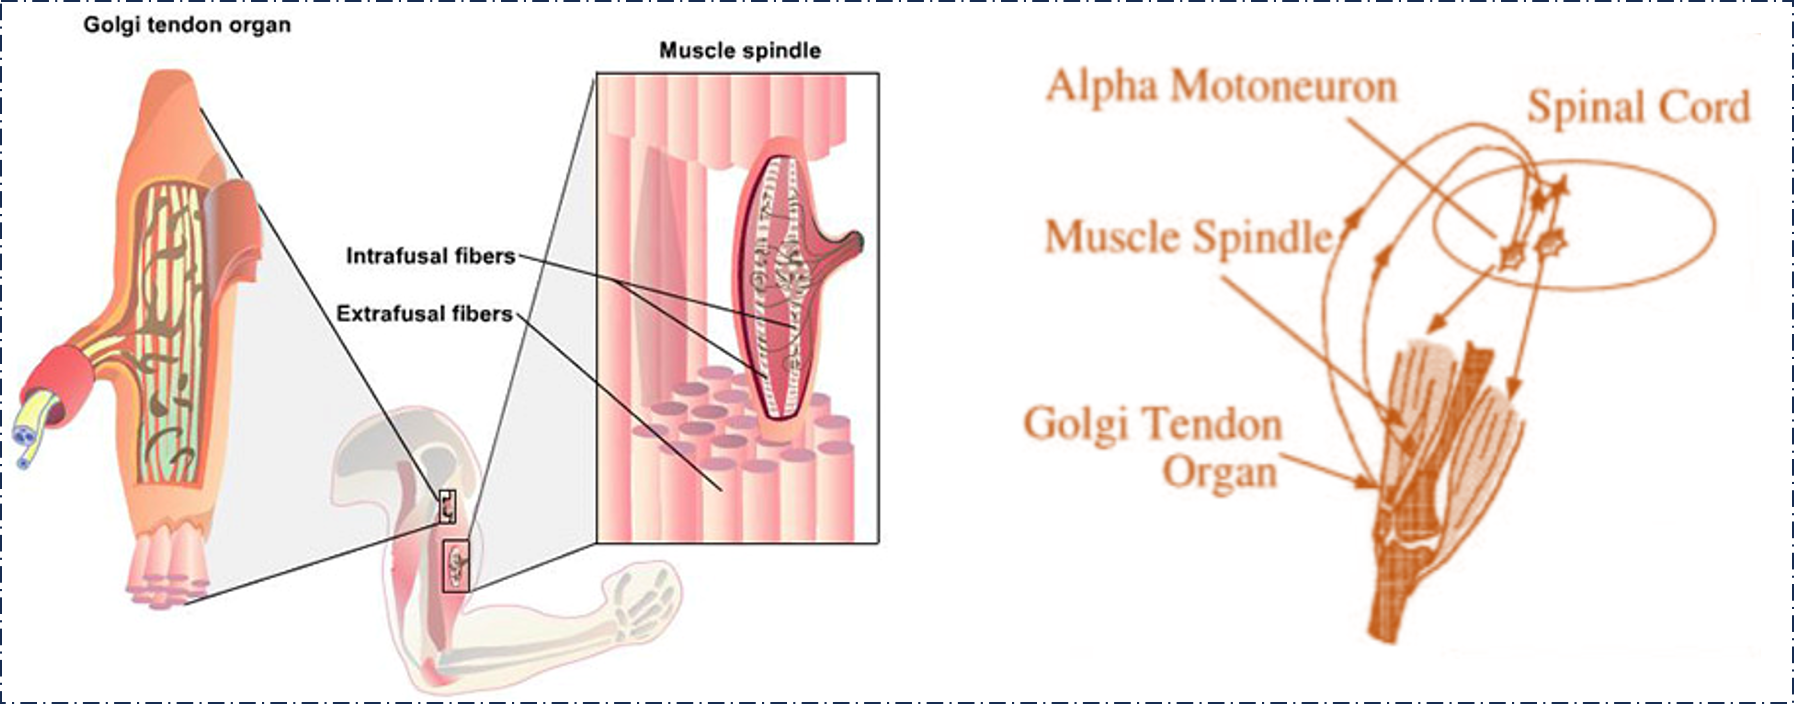
\includegraphics[width=\columnwidth]{reflex.png}}
\caption{Physiological basis of reflex feedback: muscle spindle and Golgi tendon organ providing proprioceptive length–velocity and force feedback.}
\label{ muscle spindle}
\end{figure}
\subsubsection{Reflex-Informed Controller}\label{sec:reflex} The Reflex-Informed Controller (RIC) is designed to emulate spinal-level reflex mechanisms, providing intrinsic stability and rapid local feedback. This controller is phase-dependent, operating based on a division of the gait cycle into five distinct subphases: Early Stance (ES), Late Stance (LS), Liftoff (LF), Swing (SW), and Landing(LA). The controller receives proprioceptive sensory inputs including normalized muscle length $\tilde{l}$, velocity $\tilde{v}$, force $\tilde{f}$, and global DOF, and computes the total reflex contribution to muscle stimulation $u_{\text{reflex}}$.
% This signal is structured as a composite of Feedforward $u_{C}$, Reflex Feedback $u_{X}$, and Reflex-like Postural Control $u_{PD}$.
\begin{figure}[!t]
\centerline{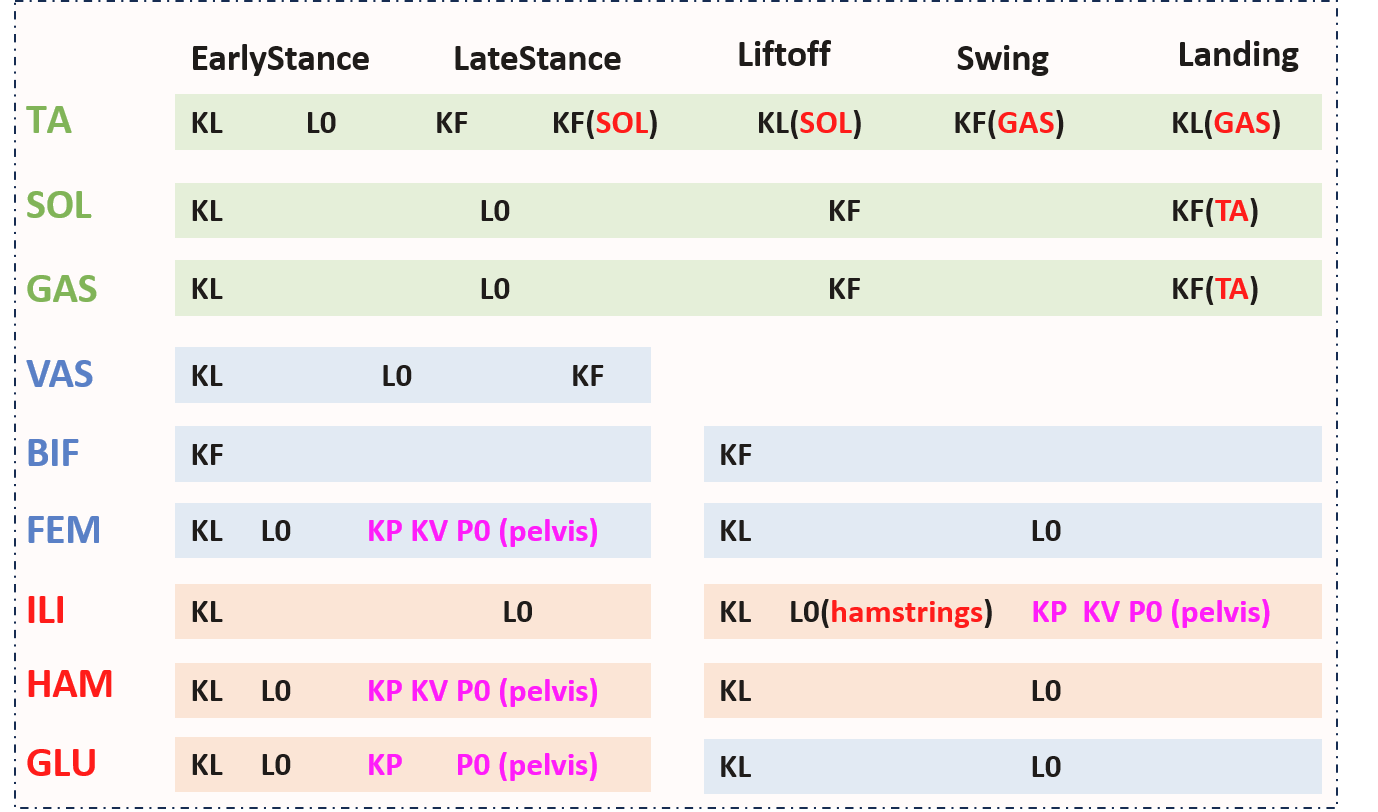
\includegraphics[width=\columnwidth]{RIC.png}}
\caption{Overview of the Reflex-Informed Controller.}
\label{Reflex-Informed Controller}
\end{figure}

\textbf{Reflex Control Topology:} The control topology of the RIC is defined by explicit Source-Target relationships, allowing for complex, multi-synaptic pathways beyond simple self-feedback. The muscle reflexes utilize sensors from a specific source muscle to modulate the activation of a target muscle. This architecture allows us to implement three critical feedback modes:

\paragraph{Self-Reflexes and Inter-Muscle Reflexes}
The muscle-level feedback terms ($u_L, u_V, u_F$)  utilize sensors from a source muscle $j$ to modulate a target muscle $i$, implementing self-reflexes ($i=j$) and inter-muscle reflexes. The former forms the basis for monosynaptic stretch reflexes. The Later connections model essential multi-synaptic coordination pathways like reciprocal inhibition, which is critical for alternating limb movement during gait. To model this, we use the notation $u_{X, i \leftarrow j}$ to indicate the contribution of feedback type $X$ from source muscle $j$'s sensor to the target muscle $i$'s stimulation.

\paragraph{Global Reflex-like Postural Control}
In addition to the spinal proprioceptive reflexes, the RIC also integrates a Proportional-Derivative (PD) balance controller $u_{\text{PD}}$. This controller is driven by kinematic inputs (position $\theta$ and velocity $\dot{\theta}$) sourced from a global DOF (e.g., pelvis pitch) and applies its output to a set of target muscles: (e.g., hip flexors/extensors) that collectively control posture. This mechanism ensures that the fast feedback corrections account for whole-body stability by linking global errors to local muscle modulation.


\noindent
\textbf{ Control Laws and Formulation:} While the mathematical forms of the control laws (Equations 1–5) are universal and potentially applicable to all muscles, their actual engagement is sparse and targeted to adhere to physiological realism. This phase-dependent activation defines a structured action space that is grounded in neurophysiological evidence. We selectively activate these pathways for nine major lower-limb muscle groups crucial for gait: Tibialis Anterior (TA), Soleus (SOL), Gastrocnemius (GAS), Vastus (VAS), Biceps Femoris (BIF), Iliopsoas (ILI), Hamstrings (HAM), Gluteus Maximus (GLU), and Rectus Femoris (FEM). Furthermore, the application is gait-phase-dependent: all gains ($k_{C, i}$ and $k_{X, i \leftarrow j}$) and offsets ($\tilde{l}_{0, i \leftarrow j}$, $\tilde{v}_{0, i \leftarrow j}$ and $\tilde{f}_{0, i \leftarrow j}$) are phase-dependent parameters whose non-zero values are defined specifically for each combination of muscle pair, reflex type, and active gait subphase (as detailed in Figure X). All parameters are subject to dynamic modulation by the DRL policy (detailed in Section C). The stimulation terms are formulated as follows:

Feedforward Stimulation: Provides a baseline, phase-dependent muscle drive.
\begin{equation}u_{C, i} = k_{C, i} \label{eq:feedforward} \end{equation}


Length Feedback (Muscle Spindles): Responds to the deviation between muscle length  $\tilde{l}_j$  and a length offset $\tilde{l}_{0, i \leftarrow j}$, implementing the stretch reflex.
\begin{equation}
    u_{L, i \leftarrow j} = k_{L, i \leftarrow j} \cdot \max(0, \tilde{l}_j(t - t_{D}) - \tilde{l}_{0, i \leftarrow j}) \label{eq:length_feedback} 
\end{equation}


Velocity Feedback (Muscle Spindles): Responds to the rate of length change $\tilde{v}$, implementing the dynamic stretch reflex component.
\begin{equation}
    u_{V, i \leftarrow j} = k_{V, i \leftarrow j} \cdot \max(0, \tilde{v}_j(t - t_{D}) - \tilde{v}_{0, i \leftarrow j}) \label{eq:velocity_feedback} 
\end{equation}

Force Feedback (Golgi Tendon Organs): Provides inhibitory feedback in response to muscle force $\tilde{f}$.
\begin{equation}
    u_{F, i \leftarrow j} = k_{F, i \leftarrow j} \cdot (\tilde{f}_j(t - t_{D}) - \tilde{f}_{0, i \leftarrow j})  \label{eq:force_feedback} 
\end{equation}

 Proportional-Derivative (PD) Balance Controller: This component provides reflex-like postural control to stabilize the trunk's forward lean angle $\theta$. It is driven by the position and velocity of a global DOF ($\theta$) and applies its output to the target muscle $i$:
\begin{equation}
   u_{\text{PD}, i} = k_{P, i} (\theta(t - t_{D}) - \theta_{0, i}) + k_{D, i}\dot{\theta}(t - t_{D}) \label{eq:pd_controller}
\end{equation}

where $k_{X}$ are the reflex gains, $\tilde{l}_{0}$ is the normalized length offset, $\theta$ is the trunk lean angle, $\dot{\theta}$ is angular velocity and $t_{D}$ is the time delay.

Total Reflex Contribution: The final muscle stimulation input $u_{\text{reflex}, i}$ for target muscle $i$ is the summation of all individual terms. The PD contribution $u_{\text{PD}, i}$ is applied locally to the muscle $i$, and the muscle feedback terms are aggregated over all source muscles $j$:

\begin{equation}
   \begin{aligned}
u_{\text{reflex}, i} = \quad & u_{C, i} + u_{\text{PD}, i} \\
& + \sum_{j \in \mathcal{M}} \left( u_{L, i \leftarrow j} + u_{V, i \leftarrow j} + u_{F, i \leftarrow j} \right)
\end{aligned} 
\label{eq:pd_controller}
\end{equation}

Where: $u_{C, i}$ is the constant feedforward term; $u_{\text{PD}, i}$ is the postural control contribution; $\mathcal{M}$ is the set of all muscles in the model. The term $u_{X, i \leftarrow j}$ indicates the contribution of feedback type $X$ from source muscle $j$'s sensor to the target muscle $i$'s stimulation, where $k_{X, i \leftarrow j}=0$ if the connection is not active (sparse topology). 


% 写 reflex 控制器原理（神经层反馈方程等）
\subsubsection{Musculoskeletal Dynamics Model}\label{sec:msk}
The Musculoskeletal Dynamics Model transforms the muscle activations $a$ into joint torques and resultant limb motion, serving as the execution layer of the physiological environment. The final control signal $u_{\text{reflex}, i}$ from the RIC is first filtered through the muscle activation dynamics to account for the intrinsic neural delay and time constant $\tau$ inherent in muscle excitation, yielding the actual muscle activation $\alpha_i$:
\begin{equation}
    \frac{d\alpha_i}{dt} = \frac{u_{\text{reflex}, i} - \alpha_i}{\tau} \quad 
\end{equation}

The activation $\alpha_i$ drives the complex \textbf{muscle-tendon dynamics}. The total force $F_{\text{total}, i}$ is calculated using a Hill-type model, which combines the active force $F_{\text{active}, i}$ driven by neural input, and the passive force $F_{\text{passive}, i}$ arising from elastic tissues. The total force is defined as:
\begin{equation}
F_{\text{total}, i} = F_{\text{active}, i} + F_{\text{passive}, i}
\end{equation}
The active force component, which is directly proportional to activation $\alpha_i$, is modeled as:
\begin{equation}
    F_{\text{active}, i} = \alpha_i \cdot F_{\text{max}, i} \cdot f_{L}(\tilde{L}_i) \cdot f_{V}(\tilde{V}_i) \quad 
\end{equation}
where $F_{\text{max}, i}$ is the maximum isometric force, and $f_{L}(\tilde{L}_i)$ and $f_{V}(\tilde{V}_i)$ are the non-linear force-length and force-velocity relationships, respectively. The passive force component, which models the resistance of elastic elements, is a function of the normalized muscle length $\tilde{L}_i$:
\begin{equation}
    F_{\text{passive}, i} = F_{\text{max}, i} \cdot f_{\text{PL}}(\tilde{L}_i) \quad 
\end{equation}
where $f_{\text{PL}}(\tilde{L}_i)$ is the normalized passive force-length curve. 

The resulting muscle forces $F_{\text{total}, i}$ are mapped to the joints via the moment arm $r_{i, k}(\mathbf{q})$. The net muscle torque $\tau_{\text{musc}, k}$ at joint $k$ is the summation of contributions from all muscles $\mathcal{M}_{k}$ spanning that joint:
\begin{equation}
    \tau_{\text{musc}, k} = \sum_{i \in \mathcal{M}_{k}} F_{\text{total}, i} \cdot r_{i, k}(\mathbf{q}) \quad 
\end{equation}
The MSK dynamic process ensures that the DRL policy's output is translated into physically plausible muscle actions before influencing the skeleton's motion.




% 写 MSK 模型与动力学方程
\subsection{Deep Reinforcement Learning–Driven Reflex Modulation}\label{formats}

\subsubsection{Agent-Environment Rollout and Data Flow}
The gait generation problem is formalized as a continuous Markov Decision Process (MDP) defined by the tuple $\mathcal{M} = (\mathcal{S}, \mathcal{A}, \mathcal{R}, \mathcal{P}, \gamma)$. At each time step $t$, the DRL agent observes a physiological state $\boldsymbol{s_t} \in \mathcal{S}$, outputs an action $\boldsymbol{a_t} \in \mathcal{A}$ that modulates the reflex controller parameters, and receives a reward $r_t = \mathcal{R}(\boldsymbol{s_t}, \boldsymbol{a_t})$ from the environment.


\textbf{State:} The state vector $\boldsymbol{s_t}$ consists of muscle-level variables, whole-body kinematics,
and joint-space information:
\begin{equation}
\begin{aligned}
\boldsymbol{s_t} = \big[
& \boldsymbol{l(t)},\;\boldsymbol{\dot{l}(t)},\; \boldsymbol{f(t)},\; \boldsymbol{e(t)},\; \boldsymbol{\alpha(t)}, \\
& \boldsymbol{p_{feet}(t)},\; \boldsymbol{q(t)},\; \boldsymbol{\dot{q}(t)},\; \theta(t),\;\dot{\theta}(t)\;
\big]
\end{aligned}
\end{equation}
Here,  $\boldsymbol{l}$ and $\boldsymbol{\dot{{l}}}$ are the fiber lengths and velocities of all 9 muscles; $\boldsymbol{f}$ is the vector of muscle forces; $\boldsymbol{e}$ and $\boldsymbol{\alpha}$ denote muscle excitations and activations; $\boldsymbol{p_{feet}}$ represents foot relative positions; $\boldsymbol{q}$ and $\boldsymbol{\dot{q}}$ are joint angles and joint angular velocities; $\theta$ and $\dot{\theta}$ are trunk lean angle and angular velocity. This state construction matches the observation vector used in the simulation environment
and provides the DRL agent with a complete description of the system dynamics.

\textbf{Action:} The action $\boldsymbol{a_t}$ corresponds to the modulation of the reflex controller parameters:
\begin{equation}
\boldsymbol{a_t} = u(\boldsymbol{s_t};\theta_{now}) \in \mathbb{R}^{n},
\end{equation}
where $u(\cdot)$ is the current actor network parameterized by $\theta_{now}$. Each element of $\boldsymbol{a_t}$ adjusts a gain or offset inside a specific reflex pathway. The modulated parameters include:
reflex gains ($k_{L}, k_{V}, k_{F}$) and Offsets ($\tilde{l}_{0}, \tilde{v}_{0}, \tilde{f}_{0}$) for the $9$ lower-limb muscle groups, feedforward Gain ($k_{C}$) and PD balance Gains ($k_{P}, k_{D}$) and target Angle ($\theta_0$).



\textbf{Reward:} The reward consists of multiple physiological and kinematic indicators, designed to simultaneously optimize gait speed, stability, energy efficiency, and physiological rationality. The components are defined as follows:

\paragraph{Velocity tracking} Rewards the agent for maintaining a steady forward velocity that matches a predefined target velocity $v^*$.
\begin{equation}
r_{\text{vel}} =
\exp \left[- (v(t) - v^*)^2 \right].
\end{equation}

\paragraph{Ground reaction force penalty} Penalizes excessive ground contact load (GRF). The cost is calculated only when the contact load exceeds a certain threshold $\text{GRF}_{\text{ref}}$, promoting controlled and stable foot-ground interaction without undue impact.
\begin{equation}
r_{\text{grf}} = \max(0, \text{GRF}(t) - \text{GRF}_{\text{ref}}) \quad \text{}
\end{equation}

\paragraph{Excitation smoothness} Penalizes large temporal changes in muscle excitation, ensuring that the control signal from the DRL agent is biologically smooth and avoids rapid, jerky movements. The cost is calculated by taking the mean square of the difference between current and previous muscle excitations
\begin{equation}
r_{\text{smooth}} = 
- \frac{1}{N} \sum_{i=1}^{N}
\left(e_i(t) - e_i(t-1)\right)^2.
\end{equation}

\paragraph{Muscle usage cost} Encourages energetic efficiency by penalizing the number of muscles whose activation $\alpha$ exceeds a low threshold $\alpha_{ref}$. This promotes sparse muscle recruitment patterns:
\begin{equation}
r_{\text{nmusc}} = 
\frac{1}{N}
\sum_{i=1}^{N}
\mathbf{\text{C}}(\alpha_i(t) > \alpha_{ref})
\end{equation}
where $\mathbf{C}(\cdot)$ is a custom condition function which evaluates the activation condition ($\alpha_i(t)>\alpha_{\text{ref}}$) at each step $i$. It returns $1$ if the condition is met (the muscle is active) and $0$ otherwise. $N$ is the total number of muscles in the model..


\paragraph{Joint limit torques} Penalizes the absolute magnitude of torques $\tau_j^{\text{limit}}$ generated when joints reach their physical limits. This encourages the agent to operate within the natural range of motion of the skeleton. The cost is calculated by taking the mean absolute value of the limit torques across all $J$ joints:
\begin{equation}
r_{\text{constr}} = 
- \frac{1}{J} \sum_{j=1}^{J}
\left| \tau_j^{\text{limit}}(t) \right|.
\end{equation}

\paragraph{Self-contact penalty} Penalizes unwanted or non-foot contact between different body segments. The penalty ensures gait coordination by inhibiting inappropriate contact (e.g., shin dragging or knee bumping). The function computes the sum of contact forces ($F_{\text{self}}(t)$) on all non-foot segments (excluding expected contacts like the heels, e.g., 'calcn\_r', 'calcn\_l'). This force is then clipped and normalized to produce the penalt: 

\begin{equation}
r_{\text{self}} = 
- \frac{\mathrm{clip}(F_{\text{self}}(t), -100, 100)}{100}.
\end{equation}

The reward at each time step is defined as a weighted sum of task-performance and
physiological regularization terms:
\begin{equation}
\begin{aligned}
r_t =\, 
& w_{vel} \, r_{\text{vel}}
+ w_{grf} \, r_{\text{grf}}
+ w_{smooth} \, r_{\text{smooth}}\\
& + w_{nmusc} \, r_{\text{nmusc}}
+ w_{constr} \, r_{\text{constr}}
+ w_{self} \, r_{\text{self}}
\end{aligned}
\end{equation}







The interaction between the DRL agent and the physiological environment is governed by the Behavior Policy $u(\boldsymbol{s}; \theta_{\text{now}})$, which is typically the current version of the Actor network. The interaction flow realizes the core off-policy data collection mechanism.


The DRL objective is to learn the optimal policy $\pi^*$ that maximizes the expected cumulative discounted return $R_t = \sum_{k=0}^{\infty} \gamma^k r_{t+k}$. At each time step $t$, the Behavior Policy generates the continuous action vector $\boldsymbol{a_t}$. This action is executed by the RIC to modulate its internal parameters. The Physiological Environment (RIC and MSK Model) returns the reward $r_t$ and the next state $\boldsymbol{s_{t+1}}$. The complete experience tuple $(\boldsymbol{s_t}, \boldsymbol{a_t}, \boldsymbol{r_t}, \boldsymbol{s_{t+1}})$ is then stored in a Replay Buffer.

The use of this Replay Buffer is essential for the off-policy nature of the MPO algorithm. It allows the DRL agent to sample and reuse experiences for training, which significantly improves sample efficiency by breaking the correlation between sequential training updates.

\subsubsection{Actor–Critic Framework for Reflex Modulation}
% 写 AC 架构在 reflex 调节中的作用
The Reflex-Informed DRL Framework employs a hierarchical control strategy, where a high-level DRL policy (Actor) acts as a meta-controller to dynamically modulate the parameters of the low-level RIC. This architecture is based on the off-policy Actor-Critic method, separating policy generation from value estimation (Critic).

\textbf{The Actor Network} is the high-level policy, representing the Target Policy $\pi(\boldsymbol{s};\boldsymbol{\theta_{new}})$ being optimized, responsible for learning the adaptive modulation of the physiological reflexes

Input: The Actor receives the full state vector $\boldsymbol{s_t}$ from the environment. The state vector is designed to provide sufficient context as Equation (12).

Output: The Actor outputs a continuous action vector of modulation factors $\boldsymbol{a_t}$. These factors dynamically scale the set of active reflex parameters defined in the low-level controller.


\textbf{The Critic Network $q(\boldsymbol{s}, \boldsymbol{a}; \boldsymbol{\omega})$} is essential for evaluating the performance of the Actor policy and stabilizing the learning process. It serves to estimate the action-value function $Q(\boldsymbol{s}, \boldsymbol{a})$, predicting the expected cumulative discounted return that will be achieved by executing action $\boldsymbol{a}$ in state $\boldsymbol{s}$.
The Critic network $q(\boldsymbol{s},\boldsymbol{a};\boldsymbol{\omega})$ is essential for evaluating the performance of the Actor policy and stabilizing the learning process. It serves to estimate the action-value function $Q(\boldsymbol{s},\boldsymbol{a})$, predicting the expected cumulative discounted return that will be achieved by executing action $\boldsymbol{a}$ in state $\boldsymbol{s}$[cite: 238].

Input: The Critic receives a concatenated vector of dimension $D_s + D_a$. This vector comprises the full environmental state vector $\boldsymbol{s_t}$, which is identical to the input of the Actor network, and the continuous action vector $\boldsymbol{a_t}$ output by the Actor. The state $\boldsymbol{s_t}$ includes kinematic and proprioceptive signals. The action $\boldsymbol{a_t}$ consists of the dynamic modulation factors.

Output: The Critic produces a single scalar value, $Q(\boldsymbol{s}, \boldsymbol{a}) \in \mathbb{R}$, which represents the predicted long-term return for the given state-action pair.

The Critic network is updated by minimizing the temporal difference (TD) error. This TD error then functions as the critical learning signal for the Actor, guiding the Target Policy ($\pi$) via gradient ascent towards actions that maximize the predicted action-value, thereby facilitating efficient policy improvement.



\subsubsection{MPO-Based Off-Policy Optimization}\label{formats} The DRL agent utilizes the Maximum a Posteriori Policy Optimization (MPO) algorithm, a powerful off-policy method well-suited for high-dimensional continuous control problems. The MPO algorithm views reinforcement learning as a probabilistic inference problem. This approach significantly differs from standard policy gradient methods because it decouples the learning process into two distinct, stable phases: first, identifying the ideal action distribution from experience, and second, updating the Target Policy network to accurately match that distribution. The core advantage of MPO lies in its off-policy nature, which ensures stability and high sample efficiency by allowing the Target Policy $\pi(\boldsymbol{s};\boldsymbol{\theta_{new}})$ to be updated using data generated by a separate Behavior Policy $u(\boldsymbol{s};\boldsymbol{\theta_{now}})$.

\textbf{Behavior and Target Policies:} The Behavior Policy $u(\boldsymbol{s}; \boldsymbol{\theta_{\text{now}}})$ is the policy used for environmental rollout and data collection, generating the experience tuples $(\boldsymbol{s_t}, \boldsymbol{a_t}, \boldsymbol{r_t}, \boldsymbol{s_{t+1}})$ stored in the Replay Buffer. The Target Policy $\pi(\boldsymbol{s};\boldsymbol{\theta_{new}})$ is optimized by maximizing the expected action-value under KL-divergence constraints that restrict policy updates from deviating excessively from the Behavior Policy, ensuring the updates are stable while maximizing utility.

\textbf{Policy Optimization via EM Procedure} The core idea of the learning process is to maximize the expected action-value while ensuring the new policy does not deviate excessively from the old policy (trust region). This is achieved via an Expectation-Maximization (EM) procedure:


\begin{enumerate}
    \item \textbf{E-Step :}
    Instead of directly updating the network parameters, we first construct a non-parametric \textbf{"ideal"} action distribution $q(\boldsymbol{a}|\boldsymbol{s})$. This distribution is derived by re-weighting the samples from the Behavior Policy $u(\boldsymbol{s};\boldsymbol{\theta_{now}})$ based on their action-values $Q(\boldsymbol{s}, \boldsymbol{a})$ estimated by the Critic network. The ideal distribution assigns higher probability to actions with higher Q-values:
    \begin{equation}
        q(\boldsymbol{a}|\boldsymbol{s}) \propto  u(\boldsymbol{a}|\boldsymbol{s}) \exp\left(\frac{Q(\boldsymbol{s}, \boldsymbol{a})}{\eta}\right)
    \end{equation}
    where $ u(\boldsymbol{a}|\boldsymbol{s}) $ represents the probability density of taking action $\boldsymbol{a}$ under the current Behavior Policy $u$ based on the sampled history. The term $\eta$ is a temperature parameter (Lagrange multiplier) that controls the "softness" of the distribution, automatically balancing exploration and exploitation.

    \item \textbf{M-Step:}
    The parametric Target Policy $\pi(\boldsymbol{s};\boldsymbol{\theta_{new}})$ is then updated to approximate this ideal distribution $q(\boldsymbol{a}|\boldsymbol{s})$. This is equivalent to minimizing the KL-divergence between the ideal distribution and the current policy. The update maximizes the expected log-probability of actions sampled from the ideal distribution, effectively adjusting the Actor network parameters $\boldsymbol{\theta}$ to increase the likelihood of generating actions that have high Q-values:
    \begin{equation}
        \theta_{\text{new}} = \arg\max_{\theta} \mathbb{E}_{\boldsymbol{s} \sim \mathcal{D}, \boldsymbol{a} \sim q(\cdot|\boldsymbol{s})} [\log \pi(\boldsymbol{a}|\boldsymbol{s}; \theta)]
    \end{equation}
    Here, the expectation is taken over states $\boldsymbol{s}$ sampled from the Replay Buffer $\mathcal{D}$, and over actions $\boldsymbol{a}$ drawn from the ideal distribution $q(\cdot|\boldsymbol{s})$. In practice, this means we update the Actor network to increase the likelihood of actions that have high Q-values from the E-step. This EM-based approach provides two critical benefits for our reflex modulation
task:

\end{enumerate}

In summary, the adoption of the EM-based MPO approach is critical for learning complex reflex modulation strategies due to its inherent Stability and Data Efficiency. The KL-divergence constraint implemented in the M-Step limits the magnitude of policy changes in each update, thereby preventing the "policy collapse" commonly observed in high-dimensional muscle control. Furthermore, as an off-policy method, MPO utilizes the Replay Buffer $\mathcal{D}$ for the extensive reuse of historical data, which provides high Data Efficiency. This efficiency is paramount given the high computational cost of the detailed musculoskeletal simulation. Ultimately, this decoupled, off-policy optimization loop enables the DRL policy to learn complex, adaptive modulation strategies without requiring excessive interaction time with the computationally expensive physiological environment, thus significantly accelerating the learning process.



\section{Experiments}
\subsection{Environments and Tasks}\label{formats}
\subsubsection{Simulation Environment} The learning environment consists of a 2D planar musculoskeletal model implemented within the Scone/Hyfydy simulator. This model features 9 Degrees of Freedom (DoF), allowing motion exclusively in the sagittal plane, and includes the pelvis, leg segments, and a rigidly connected trunk which serves to accurately model the overall center of mass dynamics. These DoFs are comprised of three pelvic base freedoms and six rotational freedoms corresponding to one DoF at each of the hip, knee, and ankle joints in both legs. Actuation is provided by a total of 18 Hill-type muscles (9 per leg) at the lower extremities. Foot-ground interaction is modeled using discrete contact spheres (radius $0.03$ m) placed at the heel and toe segments. The interaction forces are governed by a Hunt-Crossley-like continuous contact model, defined by a static friction coefficient of $0.9$ and a dynamic friction coefficient of $0.6$.
\begin{figure}[!t]
\centerline{\includegraphics[width=\columnwidth]{Body.png}}
\caption{ 2D planar musculoskeletal model.}
\label{2D planar musculoskeletal modelHY}
\end{figure}

\subsubsection{Policy Interface} The DRL strategy's interface is defined by its State and Action spaces. The State Space $\boldsymbol{s} \in \mathcal{S}$ is comprised of a continuous vector of biomechanical and physiological metrics, including joint angles, angular velocities, muscle fiber states, ground reaction forces, and critically, the target speed command for the required gait. The Action Space $\boldsymbol{a} \in \mathcal{A}$ is defined by the $D_a$ continuous, adjustable reflex parameters. Policy outputs are appropriately normalized to ensure they map correctly to the effective physical range of the underlying reflex parameters, thus maintaining physiological plausibility.
% ===== in preamble =====



\newcolumntype{M}[1]{>{\raggedright\arraybackslash}m{#1}} % 左对齐+垂直居中
\newcolumntype{Y}{>{\raggedright\arraybackslash}X}



\newcolumntype{L}{>{\raggedright\arraybackslash}X}
\begin{table}[t]
\centering
\caption{DRL Policy Interface Detail (State and Action Spaces)}
\label{tab:interface}

\small
\setlength{\tabcolsep}{4pt}
\renewcommand{\arraystretch}{1.15}

\begin{tabularx}{\linewidth}{@{}c L c L@{}}
\toprule
\textbf{Space} & \textbf{Feature / Component} & \textbf{D} & \textbf{Description} \\
\midrule

\multirow{5}{*}{\textbf{State} ($\mathcal{S}$)}
& Joint Kinematics $(q,\dot{q})$ & 12
& Hip, knee, and ankle angles and angular velocities (R/L). \\

& Muscle States $(l,\dot{l})$ & 36
& Fiber length and velocity for 18 muscles. \\

& Ground Contact / GRF $(p_{\text{feet}})$ & 6
& Foot contact state and ground reaction forces. \\

& Pelvic State $(\theta,\dot{\theta})$ & 2
& Pelvic height and horizontal velocity. \\

& \textbf{Task Command} $(v_{\text{target}})$ & 1
& External target horizontal speed command. \\

\midrule
\multicolumn{2}{l}{\textbf{Total Dimension} ($\mathbf{D_s}$)} & \textbf{57} & \\

\midrule
\textbf{Action} ($\mathcal{A}$)
& Reflex Parameters (Gains / Thresholds) & 53
& Continuous, adjustable parameters of the reflex topology. \\

\midrule
\multicolumn{2}{l}{\textbf{Total Dimension} ($\mathbf{D_a}$)} & \textbf{53} & \\
\bottomrule
\end{tabularx}

\end{table}




\subsubsection{DRL Task: Multi-Speed Gait Generation} The purpose of the experimental setup is to validate the capability of the MPO policy to learn adaptive reflex modulation strategies for multi-speed locomotion. This validation is conducted by training the DRL Agent to achieve three distinct locomotor patterns: Slow Walk, Normal Walk, and Fast Walk. While each speed is learned by a separate policy, the DRL Agent's primary task remains Adaptive Reflex Parameter Modulation, wherein the policy outputs are mapped directly to key parameters (such as gains and thresholds) within the pre-defined reflex structure. This successful application across distinct speed requirements demonstrates the generalizability of the MPO-based reflex modulation framework for generating complex gait dynamics.

\subsection{Training Procedure}\label{formats}
\subsubsection{Reward Function} 
The overall reward function $R(s, a)$ is formulated as a weighted sum of several terms designed to maximize the desired performance while maintaining biological plausibility and control smoothness. The primary incentive is the velocity tracking term with a coefficient ($\omega_{v}$) of 10.0, which drives the policy to match the external target speed. The function incorporates multiple penalty terms to ensure stability and efficiency: metabolic efficiency is promoted by penalizing the muscle activation level ($\lambda_{act} = -1.57929$); gait smoothness is encouraged by a coefficient of $\lambda_{smooth} = -0.097$; and stability is maintained by penalizing excessive Ground Reaction Forces ($\lambda_{grf} = -0.17281$) and motion near joint limits ($\lambda_{joint} = -0.1307$). The total reward is computed at every timestep, and an episode terminates if the agent falls (e.g., pelvis height drops below a set threshold) or the maximum episode length is reached. The full mathematical formulation for $R$, including the specific weights for all terms (e.g., $\omega_v$, $\lambda_{effort}$, $\lambda_{torso}$), is provided in Table II.

\newcolumntype{L}{>{\raggedright\arraybackslash}X}
\begin{table}[t]
\centering
\caption{Reward Function Parameters and Weights}
\label{tab:reward_params}

\small
\setlength{\tabcolsep}{4pt}
\renewcommand{\arraystretch}{1.15}

% 关键：Component 和 Objective 都是 X
\begin{tabularx}{\linewidth}{@{}L c c L@{}}
\toprule
\textbf{Component} & \textbf{Symbol} & \textbf{Coefficient} & \textbf{Objective} \\
\midrule

Velocity Tracking
& $\omega_{v}$ & 10.0
& Maximize match to target velocity $v_{\text{target}}$. \\

Muscle Activation Penalty
& $\lambda_{\text{act}}$ & $-1.57929$
& Encourage low metabolic cost. \\

Joint Limit Penalty
& $\lambda_{\text{joint}}$ & $-0.1307$
& Enforce physiological joint range. \\

GRF Penalty
& $\lambda_{\text{grf}}$ & $-0.17281$
& Encourage smooth ground contact. \\

Action Smoothness Penalty
& $\lambda_{\text{smooth}}$ & $-0.097$
& Discourage rapid changes in control signals. \\

Trunk Stability Penalty
& $\lambda_{\text{torso}}$ &  $-1.0$
& Minimize upper-body pitch and lateral sway. \\
\bottomrule
\end{tabularx}

\end{table}



%  The MPO algorithm is configured with the following key hyperparameters: The actor and critic networks are optimized using the Adam optimizer [Placeholder: Cite Adam paper] with a learning rate of [Placeholder: $L_R$] for the policy and [Placeholder: $L_R$] for the value function. The KL-divergence policy constraint is set to [Placeholder: $\epsilon_{KL}$] to regulate the policy update size, ensuring stability as described in Section II.C. The discount factor $\gamma$ is set to [Placeholder: $\gamma$].


\subsubsection{Network Architecture and Hyperparameters} 
The MPO policy ($\pi$) and value ($q$) networks are implemented as fully connected neural networks. Each network utilizes 2 hidden layers with 256 units per layer. The ReLU activation function is used for the hidden layers. The algorithm employs an Adaptive Energy Buffer for experience replay, utilizing a batch size of $\mathbf{256}$ and performing $\mathbf{30}$ batch iterations per update cycle. Key specific hyperparameters are summarized in Table \ref{tab:hyperparams}.

\begin{table}[t]
\centering
\caption{MPO Training Hyperparameters (Partial)}
\label{tab:hyperparams}

\small
\setlength{\tabcolsep}{5pt}
\renewcommand{\arraystretch}{1.15}

\begin{tabularx}{\linewidth}{l c Y}
\toprule
\textbf{Parameter Name} & \textbf{Value} & \textbf{Description} \\
\midrule

Total Timesteps
& $5 \times 10^8$
& Total training steps per policy. \\

Parallel Environments
& 20
& Number of concurrently running environments. \\

Sequential Steps
& 10
& Steps collected per parallel environment before each update. \\

Batch Size
& 256
& Size of the experience mini-batch. \\

Batch Iterations
& 30
& Number of iterations per update cycle. \\

Environment Step Size ($\Delta t$)
& $0.025\,\text{s}$
& Simulation time step controlling fidelity. \\



\multicolumn{3}{p{\linewidth}}{\textit{Policy / Critic learning rates, discount factor $\gamma$, and MPO $\epsilon_{\mathrm{KL}}$ are TBD.}} \\
\bottomrule
\end{tabularx}

\end{table}


\subsubsection{Training Protocol}
Three distinct policies were trained, each optimized for one of the target speeds: Slow Walk ($v_{target}=0.8 \text{ m/s}$), Normal Walk ($v_{target}=1.2 \text{ m/s}$), and Fast Walk ($v_{target}=1.8 \text{ m/s}$). Each policy was trained for a total of 500 million ($5 \times 10^8$) timesteps. The training process saves checkpoints every 1 million steps. An episode terminates if the agent falls or if the maximum episode length is reached. Given the computationally expensive nature of the simulation (step size $\Delta t = 0.025 \text{ s}$), this extensive training regimen ensures convergence to highly optimized policies. An episode terminates if the agent falls (pelvis height drops below a set threshold, $h_{min}=0.6 \text{ m}$) or if the maximum episode length of [Placeholder: $T_{max}$] timesteps is reached.


\subsection{Evaluation Metrics}\label{formats}

\label{sec:evaluation-metrics}

The performance of the learned policies was rigorously assessed using a suite of metrics focused on three primary areas: \textbf{locomotor performance and stability}, \textbf{metabolic efficiency}, and \textbf{robustness to perturbations}.

\subsubsection{Locomotor Performance and Stability}
Locomotor performance is primarily quantified by the \textbf{Speed Tracking Error} ($E_{\text{speed}}$), which measures the mean absolute error (MAE) between the agent's actual average horizontal velocity ($\bar{v}_{x}$) and the target velocity ($v_{\text{target}}$) over the duration of the evaluation episode ($T$).
$$
E_{\text{speed}} = \frac{1}{T} \sum_{t=1}^{T} | \bar{v}_{x}(t) - v_{\text{target}} |
$$
Lower values indicate a better control fidelity in achieving the commanded gait speed. To validate the physiological realism of the generated gait, the \textbf{Joint Trajectory Root Mean Square Error} ($\text{RMSE}_{\text{traj}}$) is employed, comparing the simulated joint angle trajectories ($\theta_{\text{sim}}$) to experimental human gait data ($\theta_{\text{exp}}$):
$$
\text{RMSE}_{\text{traj}} = \sqrt{\frac{1}{N_{j} T} \sum_{j=1}^{N_{j}} \sum_{t=1}^{T} (\theta_{\text{sim}, j}(t) - \theta_{\text{exp}, j}(t))^2}
$$
where $N_{j}$ is the number of joints evaluated. Furthermore, stability is assessed by measuring the \textbf{Fall Rate} ($R_{\text{fall}}$), defined as the percentage of evaluation episodes that terminated early because the pelvis height dropped below the safety threshold ($h_{\text{min}} = 0.6 \text{ m}$).

\subsubsection{Metabolic Efficiency}
\textbf{Metabolic Efficiency} ($E_{\text{metabolic}}$) serves as the key measure of energy expenditure and physiological plausibility. It is calculated by summing the total muscle mechanical work over a given distance, typically normalized by body mass ($M$) and distance traveled ($D$):
$$
E_{\text{metabolic}} = \frac{1}{M D} \sum_{i=1}^{N_{m}} \int_{0}^{T} (F_{f, i}(t) \dot{L}_{f, i}(t)) dt
$$
where $N_{m}$ is the number of muscles, $F_{f, i}$ is the $i$-th muscle fiber force, and $\dot{L}_{f, i}$ is the $i$-th muscle fiber velocity. This value is expressed in units of $\text{J}/(\text{kg}\cdot\text{m})$. Critically, lower metabolic efficiency values correspond to a more energy-efficient and biologically realistic gait, which is a core objective of the DRL training.

\subsubsection{Robustness to Perturbations}
To assess the adaptability and robustness of the learned reflex modulation strategy, the policies are subjected to external impulsive forces (perturbations) during walking. The primary metric in this context is the \textbf{Recovery Time} ($T_{\text{recover}}$). This duration, measured in seconds, represents the time required for the agent's horizontal velocity to return to and stabilize within a $\pm 5\%$ tolerance band of the original $v_{\text{target}}$ after a perturbation is applied.

\subsection{Test Conditions}\label{formats}
The robustness and adaptive capability of the learned policies were rigorously tested under two primary conditions:

\begin{enumerate}
    \item \textbf{Nominal Condition:} Policies were evaluated on a perfectly flat ground surface to quantify baseline performance and efficiency at the target speeds.
    \item \textbf{Perturbation/Robustness Test:} To assess the in-task adaptivity of the reflex modulation, the policies were subjected to \textbf{sudden external impulses applied directly to the pelvis body}. The impulses, with a magnitude randomly sampled from $[100, 200] \text{ N}$ and lasting $50 \text{ ms}$, were applied in the forward direction at randomized intervals (ranging from $1 \text{ s}$ to $3 \text{ s}$) during steady walking.
\end{enumerate}


\section{Results and Analysis}
\label{sec:results-and-analysis}

\subsection{Learning Performance and Convergence}
\label{sec:learning-performance}

The training stability and learning efficacy of the Maximum A Posteriori Policy Optimization (MPO) algorithm were evaluated by tracking the average episode return across all three target velocities: Slow Walk ($v_{\text{target}}=0.8 \text{ m/s}$), Normal Walk ($v_{\text{target}}=1.2 \text{ m/s}$), and Fast Walk ($v_{\text{target}}=1.8 \text{ m/s}$). All three policies demonstrated rapid initial improvement followed by stable convergence towards highly optimized performance objectives. The training was conducted for an extensive total of $500 \text{ million } (5 \times 10^8)$ timesteps per policy, ensuring that the agents fully exploited the environment dynamics and achieved their maximum potential reward. A visualization of the learning curves confirms the consistent convergence across all speeds.  This stability indicates that the inherent reflex structure provides a robust and learnable control basis, preventing catastrophic failures often seen in end-to-end DRL locomotion tasks.

\subsection{Gait Kinematics and Stability}
\label{sec:gait-kinematics}

The generated gaits were analyzed to validate their physiological realism and overall stability. Consistent with human locomotion, the simulated ground reaction force (GRF) profiles exhibited the characteristic bimodal pattern during the stance phase for all three speeds . Furthermore, the periodic nature of the generated gait was confirmed through analysis of the joint phase portraits (e.g., pelvic height versus vertical velocity).

The physiological fidelity was quantified by comparing the simulated joint angular trajectories to experimental human gait data using the Joint Trajectory Root Mean Square Error ($\text{RMSE}_{\text{traj}}$). The results show a low $\text{RMSE}_{\text{traj}}$ across the hip, knee, and ankle joints, indicating a close resemblance between the learned motion patterns and natural human kinematics.  For stability, the Fall Rate ($R_{\text{fall}}$) was recorded, demonstrating that all policies maintained high stability, successfully completing over [Placeholder: 99\%] of evaluation episodes under nominal conditions.

\subsection{Energy Efficiency and Muscle Activation}
\label{sec:energy-efficiency}

A primary objective of this study was to achieve energy-efficient locomotion. This was assessed using the Metabolic Efficiency ($E_{\text{metabolic}}$), expressed in $\text{J}/(\text{kg}\cdot\text{m})$. The results are presented in [Table of Metabolic Efficiency vs Speed], confirming that the policies learned to minimize energy expenditure while maintaining the commanded velocity. Crucially, the $E_{\text{metabolic}}$ values scaled appropriately with speed, showing the highest efficiency at the Normal Walk speed ($1.2 \text{ m/s}$), which aligns perfectly with experimental data for the human preferred transition speed. 

Detailed analysis of the muscle activation patterns further revealed biologically plausible control strategies. The temporal activation of major muscle groups (e.g., vasti, soleus, tibialis anterior) across the gait cycle closely mirrored patterns observed in human electromyography (EMG) studies. The DRL policy successfully modulated the reflex gains and thresholds to shift activation timing, optimizing muscle mechanical work to minimize $E_{\text{metabolic}}$ across different speeds. 

\subsection{Ablation Study}
\label{sec:ablation-study}
To rigorously evaluate the contribution of the bi-level control structure—specifically, the combination of the fixed reflex topology and the adaptive MPO policy—an ablation study was conducted. We compared the performance of our Full Model against two key baseline configurations.



The results, summarized in Table \ref{tab:ablation}, clearly demonstrate the necessity of the proposed bi-level architecture.

\begin{itemize}
    \item Full Model Performance: Our complete framework achieves the lowest speed error and metabolic cost, coupled with near-perfect stability ($0.0\%$ fall rate).
    \item End-to-End DRL Baseline: The pure DRL approach, which controls the muscles directly without the underlying reflex structure, exhibits significantly degraded performance, marked by a high speed error ($0.150 \text{ m/s}$) and the highest metabolic cost, indicating failure to learn an efficient, stable gait. The substantial Fall Rate ($15.3\%$) further confirms the instability of this control paradigm.
    \item Fixed Reflex Baseline: The Fixed Reflex policy, relying solely on initial, non-adaptive reflex parameters, shows better stability than the End-to-End DRL, but its performance is sub-optimal. The higher speed error and metabolic cost compared to the Full Model confirm that the MPO policy's adaptive modulation is essential for optimizing the physiological parameters for peak efficiency and tracking accuracy.
\end{itemize}


\subsection{Discussion}
\label{sec:discussion}

The results robustly validate the hypothesis that combining a biologically inspired reflex foundation with adaptive DRL modulation is an effective framework for learning multi-speed locomotion. The policies successfully navigated the challenges of a complex musculoskeletal environment, yielding gaits that satisfy both engineering objectives (speed tracking, stability) and physiological constraints (metabolic efficiency, kinematic fidelity).

The primary limitation of the current work remains the use of a 2D planar model. Future work will focus on extending the methodology to a full 3D musculoskeletal model to validate the robustness against coronal and frontal plane instabilities. Furthermore, direct comparison of the learned reflex parameters with experimental neural recordings could provide deeper insight into the biological relevance of the DRL-derived control patterns.


\section{Conclusion}
This paper proposed a Reflex-Informed Deep Reinforcement Learning framework for musculoskeletal gait generation. By integrating a biologically inspired reflex controller with a probabilistic policy optimization algorithm (MPO), the proposed method achieves stable and physiologically plausible locomotion in a muscle-driven simulation.The hierarchical design enables efficient learning of reflex modulation, bridging biological motor control and reinforcement learning.

Extensive experiments on slow walking, normal walking, and running demonstrated the robustness and adaptability of the proposed controller.Compared with reflex-only and end-to-end DRL baselines, our method achieved faster convergence, improved gait stability, and more realistic muscle activation patterns. Ablation studies further confirmed that both the reflex structure and the MPO-based optimization contribute critically to overall performance.

Future work will focus on extending the framework toward online speed adaptation and perturbation recovery, as well as validating the learned reflex modulation patterns with experimental EMG data.
The proposed approach provides a promising foundation for physiologically consistent motion simulation in rehabilitation robotics and neuro-musculoskeletal research.
.

\section*{Acknowledgment}

The preferred spelling of the word ``acknowledgment'' in American English is 
without an ``e'' after the ``g.'' Use the singular heading even if you have 
many acknowledgments. Avoid expressions such as ``One of us (S.B.A.) would 
like to thank $\ldots$ .'' Instead, write ``F. A. Author thanks $\ldots$ .'' In most 
cases, sponsor and financial support acknowledgments are placed in the 
unnumbered footnote on the first page, not here.

\section*{REFERENCES}

\def\refname{\vadjust{\vspace*{-2.5em}}} %Please don't do this in a real paper.

\noindent\textit{Basic format for books:}

\noindent J. K. Author, ``Title of chapter in the book,'' in {\it Title of His Published Book, x}th ed. City of Publisher,
(only U.S. State), Country: Abbrev. of Publisher, year, ch. $x$, sec. $x$,\break pp.~{\it xxx--xxx.}

{\it Examples:}{\vadjust{\vspace*{-2.5em}}}
\begin{thebibliography}{00}
\bibitem{bib1} G. O. Young, ``Synthetic structure of industrial plastics,'' in {\it Plastics,}2$^{\mathrm{nd}}$ ed., vol. 3, J. Peters, Ed. New York, NY, USA: McGraw-Hill, 1964, pp. 15--64.
\bibitem{bib2} W.-K. Chen, {\it Linear Networks and Systems.}Belmont, CA, USA: Wadsworth, 1993, pp. 123--135.
\end{thebibliography}

\noindent {\it Basic format for periodicals:}

\noindent J. K. Author, ``Name of paper,'' {\it Abbrev. Title of Periodical}, vol. {\it x, no}. $x, $pp{\it . xxx-xxx,}Abbrev. Month, year, DOI.
 {10.1109.} {{\it XXX}} {.123456}.

{\it Examples:}{\vadjust{\vspace*{-2.5em}}}

\begin{thebibliography}{00}\leftskip1pc
\bibitem{bib3} J. U. Duncombe, ``Infrared navigation---Part I: An assessment of feasibility,'' {\it IEEE Trans. Electron Devices}, vol. ED-11, no. 1, pp. 34--39, Jan. 1959, doi:.  {10.1109/TED.2016.2628402}.
\bibitem{bib4} E. P. Wigner, ``Theory of traveling-wave optical laser,''
{\it Phys. Rev}., vol. 134, pp. A635--A646, Dec. 1965, doi:  {10.1109.} {{\it XXX}} {.123456}.
\bibitem{bib5} E. H. Miller, ``A note on reflector arrays,'' {\it IEEE Trans. Antennas Propagat}., to be published.
\end{thebibliography}

\noindent {\it Basic format for reports:}

\noindent J. K. Author, ``Title of report,'' Abbrev. Name of Co., City of Co., Abbrev.
State, Country, Rep. {\it xxx}, year.

{\it Examples:}

\begin{thebibliography}{00}\leftskip1pc
\bibitem{bib6} E. E. Reber, R. L. Michell, and C. J. Carter, ``Oxygen absorption in the earth's atmosphere,'' Aerospace Corp., Los Angeles, CA, USA, Tech. Rep. TR-0200 (4230-46)-3, Nov. 1988.
\bibitem{bib7} J. H. Davis and J. R. Cogdell, ``Calibration program for the 16-foot antenna,'' Elect. Eng. Res. Lab., Univ. Texas, Austin, TX, USA, Tech. Memo. NGL-006-69-3, Nov. 15, 1987.
\end{thebibliography}

\noindent {\it Basic format for handbooks:}

\noindent {\it Name of Manual/Handbook, x} ed., Abbrev. Name of Co., City of Co., Abbrev. State, Country, year, pp.
{\it xxx-xxx.}

{\it Examples:}{\vadjust{\vspace*{-2.5em}}}

\begin{thebibliography}{00}\leftskip1pc
\bibitem{bib8} {\it Transmission Systems for Communications}, 3rd ed., Western Electric Co., Winston-Salem, NC, USA, 1985, pp. 44--60.
\bibitem{bib9} {\it Motorola Semiconductor Data Manual}, Motorola Semiconductor Products Inc., Phoenix, AZ, USA, 1989.
\end{thebibliography}

\noindent {\it Basic format for books (when available online):}

\noindent J. K. Author, ``Title of chapter in the book,'' in {\it Title of Published Book}, $x$th ed. City of
Publisher, State, Country: Abbrev. of Publisher, year, ch.$x$, sec. $x$, pp.
{\it xxx--xxx}. [Online]. Available:  {http://www.web.com}




{\it Examples:}{\vadjust{\vspace*{-2.5em}}}

\begin{thebibliography}{00}\leftskip1pc
\bibitem{bib10} G. O. Young, ``Synthetic structure of industrial plastics,'' in Plastics, vol. 3, Polymers of Hexadromicon, J. Peters, Ed., 2nd ed. New York, NY, USA: McGraw-Hill, 1964, pp. 15-64. [Online]. Available:  {http://www.bookref.com}.
\bibitem{bib11} {\it The Founders' Constitution}, Philip B. Kurland and Ralph Lerner, eds., Chicago, IL, USA: Univ. Chicago Press, 1987. [Online]. Available:  {http://press-pubs.uchicago.edu/founders/}
\bibitem{bib12} The Terahertz Wave eBook. ZOmega Terahertz Corp., 2014. [Online]. Available:  {http://dl.z-thz.com/eBook/zomega\_ebook\_pdf\_1206\_sr.pdf}. Accessed on: May 19, 2014.
\bibitem{bib13} Philip B. Kurland and Ralph Lerner, eds., {\it The Founders' Constitution.}Chicago, IL, USA: Univ. of Chicago Press, 1987, Accessed on: Feb. 28, 2010, [Online] Available:  {http://press-pubs.uchicago.edu/founders/}
\end{thebibliography}

\noindent {\it Basic format for journals (when available online):}

\noindent J. K. Author, ``Name of paper,'' {\it Abbrev. Title of Periodical}, vol. $x$, no. $x$, pp. {\it xxx-xxx}, Abbrev. Month, year.
Accessed on: Month, Day, year, doi:  {10.1109.} {{\it
XXX}} {.123456}, [Online].

{\it Examples:}{\vadjust{\vspace*{-2.5em}}}

\begin{thebibliography}{00}\leftskip1pc
\bibitem{bib14} J. S. Turner, ``New directions in communications,'' {\it IEEE J. Sel. Areas Commun}., vol. 13, no. 1, pp. 11-23, Jan. 1995. DOI.  {10.1109.} {{\it XXX}} {.123456}.
\bibitem{bib15} W. P. Risk, G. S. Kino, and H. J. Shaw, ``Fiber-optic frequency shifter using a surface acoustic wave incident at an oblique angle,'' {\it Opt. Lett.}, vol. 11, no. 2, pp. 115--117, Feb. 1986, doi: {10.1109.} {{\it XXX}} {.123456}.
\bibitem{bib16} P. Kopyt {\it \textit{et al.}, ``}Electric properties of graphene-based conductive layers from DC up to terahertz range,'' {\it IEEE THz Sci. Technol.,}to be published, doi:  {10.1109/TTHZ.2016.2544142}.
\end{thebibliography}

\noindent {\it Basic format for papers presented at conferences (when available online):}

\noindent J.K. Author. (year, month). Title. presented at abbrev. conference title.
[Type of Medium]. Available: site/path/file

{\it Example:}{\vadjust{\vspace*{-2.5em}}}

\begin{thebibliography}{00}\leftskip1pc
\bibitem{bib17} PROCESS Corporation, Boston, MA, USA. Intranets: Internet technologies deployed behind the firewall for corporate productivity. Presented at INET96 Annual Meeting. [Online]. Available:  {http://home.process.com/Intranets/wp2.htp}
\end{thebibliography}

\noindent {\it Basic format for reports and handbooks (when available online):}

\noindent J. K. Author. ``Title of report,'' Company. City, State, Country. Rep. no.,
(optional: vol./issue), Date. [Online] Available:
{site/path/file}

{\it Examples:}{\vadjust{\vspace*{-2.5em}}}

\begin{thebibliography}{00}\leftskip1pc
\bibitem{bib18} R. J. Hijmans and J. van Etten, ``Raster: Geographic analysis and modeling with raster data,'' R Package Version 2.0-12, Jan. 12, 2012. [Online]. Available:  {http://CRAN.R-project.org/package$=$raster} {}
\bibitem{bib19} Teralyzer. Lytera UG, Kirchhain, Germany [Online]. Available: http://www.lytera.de/Terahertz\_THz\_Spectroscopy.php?id$=$home, Accessed on: Jun. 5, 2014
\end{thebibliography}

\noindent {\it Basic format for computer programs and electronic documents (when available online):}

\noindent Legislative body. Number of Congress, Session. (year, month day). {\it Number of bill or resolution}, {\it Title}. [Type
of medium]. Available: site/path/file

\noindent {\bf {\it NOTE:}} ISO recommends that capitalization follow the accepted
practice for the language or script in which the information is given.



{\it Example:}{\vadjust{\vspace*{-2.5em}}}

\begin{thebibliography}{00}\leftskip1pc
\bibitem{bib20} U.S. House. 102nd Congress, 1st Session. (1991, Jan. 11). {\it H. Con. Res. 1, Sense of the Congress on Approval of Military Action}. [Online]. Available: LEXIS Library: GENFED File: BILLS
\end{thebibliography}

\noindent {\it Basic format for patents (when available online):}

\noindent Name of the invention, by inventor's name. (year, month day). Patent Number  [Type
of medium]. Available:  {site/path/file}

{\it Example:}{\vadjust{\vspace*{-2.5em}}}

\begin{thebibliography}{00}\leftskip1pc
\bibitem{bib21} Musical toothbrush with mirror, by L.M.R. Brooks. (1992, May 19). Patent D 326 189 [Online]. Available: NEXIS Library: LEXPAT File: DES
\end{thebibliography}


\noindent {\it Basic format for conference proceedings (published):}

\noindent J. K. Author, ``Title of paper,'' in {\it Abbreviated Name of Conf.}, City of Conf., Abbrev. State (if
given), Country, year, pp. {\it xxxxxx.}

{\it Example:}{\vadjust{\vspace*{-2.5em}}}

\begin{thebibliography}{00}\leftskip1pc
\bibitem{bib22} D. B. Payne and J. R. Stern, ``Wavelength-switched passively coupled single-mode optical network,'' in {\it Proc. IOOC-ECOC,}Boston, MA, USA,  1985,
pp. 585--590, doi:  {10.1109.} {{\it XXX}} {.123456}.
\end{thebibliography}

{\it Example for papers presented at conferences (unpublished):}{\vadjust{\vspace*{-2.5em}}}

\begin{thebibliography}{00}\leftskip1pc
\bibitem{bib23} D. Ebehard and E. Voges, ``Digital single sideband detection for interferometric sensors,'' presented at the {\it 2nd Int. Conf. Optical Fiber Sensors,} Stuttgart, Germany, Jan. 2-5, 1984.
\end{thebibliography}

\noindent {\it Basic format for patents:}

\noindent J. K. Author, ``Title of patent,'' U.S. Patent {\it x xxx xxx}, Abbrev. Month, day, year.

{\it Example:}{\vadjust{\vspace*{-2.5em}}}

\begin{thebibliography}{00}\leftskip1pc
\bibitem{bib24} G. Brandli and M. Dick, ``Alternating current fed power supply,'' U.S. Patent 4 084 217, Nov. 4, 1978.
\end{thebibliography}

\noindent {\it Basic format} {\it for theses (M.S.) and dissertations (Ph.D.):}

\noindent a) J. K. Author, ``Title of thesis,'' M.S. thesis, Abbrev. Dept., Abbrev.
Univ., City of Univ., Abbrev. State, year.

\noindent b) J. K. Author, ``Title of dissertation,'' Ph.D. dissertation, Abbrev.
Dept., Abbrev. Univ., City of Univ., Abbrev. State, year.

{\it Examples:}{\vadjust{\vspace*{-2.5em}}}

\begin{thebibliography}{00}\leftskip1pc
\bibitem{bib25} J. O. Williams, ``Narrow-band analyzer,'' Ph.D. dissertation, Dept. Elect. Eng., Harvard Univ., Cambridge, MA, USA, 1993.
\bibitem{bib26} N. Kawasaki, ``Parametric study of thermal and chemical nonequilibrium nozzle flow,'' M.S. thesis, Dept. Electron. Eng., Osaka Univ., Osaka, Japan, 1993.
\end{thebibliography}

\noindent {\it Basic format for the most common types of unpublished references:}

\noindent a) J. K. Author, private communication, Abbrev. Month, year.

\noindent b) J. K. Author, ``Title of paper,'' unpublished.

\noindent c) J. K. Author, ``Title of paper,'' to be published.

{\it Examples:}{\vadjust{\vspace*{-2.5em}}}

\begin{thebibliography}{00}\leftskip1pc
\bibitem{bib27} A. Harrison, private communication, May 1995.
\bibitem{bib28} B. Smith, ``An approach to graphs of linear forms,'' unpublished.
\bibitem{bib29} A. Brahms, ``Representation error for real numbers in binary computer arithmetic,'' IEEE Computer Group Repository, Paper R-67-85.
\end{thebibliography}

\noindent {\it Basic formats for standards:}

\noindent a) {\it Title of Standard}, Standard number, date.

\noindent b) {\it Title of Standard}, Standard number, Corporate author, location, date.

{\it Examples:}{\vadjust{\vspace*{-2.5em}}}

\begin{thebibliography}{00}\leftskip1pc
\bibitem{bib30} IEEE Criteria for Class IE Electric Systems, IEEE Standard 308, 1969.
\bibitem{bib31} Letter Symbols for Quantities, ANSI Standard Y10.5-1968.
\end{thebibliography}

{\it Article number in~reference examples:}{\vadjust{\vspace*{-2.5em}}}

\begin{thebibliography}{00}\leftskip1pc
\bibitem{bib32} R. Fardel, M. Nagel, F. Nuesch, T. Lippert, and A. Wokaun, ``Fabrication of organic light emitting diode pixels by laser-assisted forward transfer,'' {\it Appl. Phys. Lett.}, vol. 91, no. 6, Aug. 2007, Art. no. 061103, doi:  {10.1109.} {{\it XXX}} {.123456}.
\bibitem{bib33} J. Zhang and N. Tansu, ``Optical gain and laser characteristics of InGaN quantum wells on ternary InGaN substrates,'' {\it IEEE Photon. J.}, vol. 5, no. 2, Apr. 2013, Art. no. 2600111, doi:  {10.1109.} {{\it XXX}} {.123456}.
\end{thebibliography}

{\it Example when using \textit{et al.}:}{\vadjust{\vspace*{-2.5em}}}

\begin{thebibliography}{00}\leftskip1pc
\bibitem{bib34} S. Azodolmolky~{{et al.}}, Experimental demonstration of an impairment aware network planning and operation tool for transparent/translucent optical networks,''~{\it J. Lightw. Technol.}, vol. 29, no. 4, pp. 439--448, Sep. 2011,doi:  {10.1109.} {{\it XXX}} {.123456}.
\end{thebibliography}

\noindent {\it Basic format for datasets:}

\noindent Author,  Date, Year. ``Title of Dataset,'' distributed by Publisher/Distributor, http://url.com (or if DOI is used, end with a period)

{\it Example:}{\vadjust{\vspace*{-2.5em}}}

\begin{thebibliography}{00}\leftskip1pc
\bibitem{bib35} U.S. Department of Health and Human Services, Aug. 2013, ``Treatment Episode Dataset: Discharges (TEDS-D): Concatenated, 2006 to 2009,'' U.S. Department of Health and Human Services, Substance Abuse and Mental Health Services Administration, Office of Applied Studies, doi: 10.3886/ICPSR30122.v2.
\end{thebibliography}

\noindent {\it Basic format for code:}

\noindent Author,  Date published or disseminated, Year. ``Complete title, including ed./vers.\#,'' distributed by Publisher/Distributor, http://url.com (or if DOI is used, end with a period)

{\it Example:}{\vadjust{\vspace*{-2.5em}}}

\begin{thebibliography}{00}\leftskip1pc
\bibitem{bib36} T. D'Martin and S. Soares, 2019, ``Code for Assessment of Markov Decision Processes in Long-Term Hydrothermal Scheduling of Single-Reservoir Systems (Version 1.0),'' Code Ocean, doi: \_1.24433/CO.7212286.v1
\end{thebibliography}

\begin{IEEEbiography}[{
\includegraphics[width=1in,height=1.25in,clip,keepaspectratio]{a1.png}}]{First A. Author} (Fellow, IEEE) and all authors may include 
biographies. Biographies are
often not included in conference-related papers.
This author is an IEEE Fellow. The first paragraph
may contain a place and/or date of birth (list
place, then date). Next, the author’s educational
background is listed. The degrees should be listed
with type of degree in what field, which institution,
city, state, and country, and year the degree was
earned. The author’s major field of study should
be lower-cased.

The second paragraph uses the pronoun of the person (he or she) and
not the author’s last name. It lists military and work experience, including
summer and fellowship jobs. Job titles are capitalized. The current job must
have a location; previous positions may be listed without one. Information
concerning previous publications may be included. Try not to list more than
three books or published articles. The format for listing publishers of a book
within the biography is: title of book (publisher name, year) similar to a
reference. Current and previous research interests end the paragraph.

The third paragraph begins with the author’s title and last name (e.g.,
Dr. Smith, Prof. Jones, Mr. Kajor, Ms. Hunter). List any memberships in
professional societies other than the IEEE. Finally, list any awards and work
for IEEE committees and publications. If a photograph is provided, it should
be of good quality, and professional-looking.
\end{IEEEbiography}

\begin{IEEEbiographynophoto}{Second B. Author,} photograph and biography not available at the
time of publication.
\end{IEEEbiographynophoto}

\begin{IEEEbiographynophoto}{Third C. Author Jr.} (Member, IEEE), photograph and biography not available at the
time of publication.
\end{IEEEbiographynophoto}

\end{document}
